\pagebreak
\section{Standard Coordinate Spaces}
\label{sect:StdCoordSpaces}
We provide standard instances of commonly used coordinate spaces as instances of elements from this model.  Each element has a formal identifier (ID) which can be used to reference the instance given here.

  \subsection{Standard Cartesian Coordinate Space}
  \label{sect:Cartesian}

  \begin{minipage}{0.5\textwidth}
    \small
    \textbf{id}: \_CARTESIAN\_CoordSpace \newline
    Coordinate space comprised of 3 orthogonal axes.
    
    \noindent \textbf{Axis1} \newline
    \indent id:  \_CARTESIAN\_X\_Axis \newline
    \indent domainMin:  -Infinity \newline
    \indent domainMax:  +Infinity \newline
    \indent cyclic:  False \newline
    
    \noindent \textbf{Axis2} \newline
    \indent id:  \_CARTESIAN\_Y\_Axis \newline
    \indent domainMin:  -Infinity \newline
    \indent domainMax:  +Infinity \newline
    \indent cyclic:  False \newline
    
    \noindent \textbf{Axis3} \newline
    \indent id:  \_CARTESIAN\_Z\_Axis \newline
    \indent domainMin:  -Infinity \newline
    \indent domainMax:  +Infinity \newline
    \indent cyclic:  False \newline
    \normalsize
  \end{minipage}
  \begin{minipage}{0.5\textwidth}
    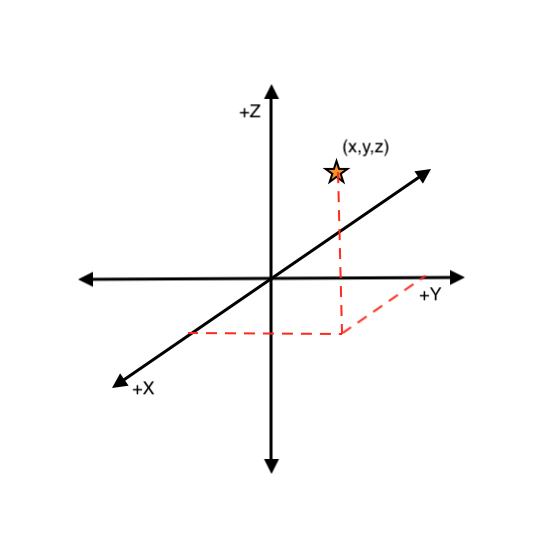
\includegraphics{diagrams/CartesianSpace.png}
  \end{minipage}
  \vspace{-0.75cm}

  \subsection{Standard Spherical Coordinate Space}
  \label{sect:Spherical}

  \begin{minipage}{0.5\textwidth}
    \small
    \textbf{id}: \_SPHERICAL\_CoordSpace \newline
    A 3 dimensional spherical coordinate space, comprised of 2 angular axes and 1 radial axis.
    
    \noindent \textbf{Axis1} \newline
    \indent id:  \_SPHERICAL\_Lat\_Axis \newline
    \indent domainMin:  -90.0 deg \newline
    \indent domainMax:  +90.0 deg \newline
    \indent cyclic: False \newline
    
    \noindent \textbf{Axis2} \newline
    \indent id:  \_Spherical\_Long\_Axis \newline
    \indent domainMin: 0.0 deg \newline
    \indent domainMax: 360.0 deg \newline
    \indent cyclic: True \newline
    
    \noindent \textbf{Axis3} \newline
    \indent id:  \_Spherical\_R\_Axis \newline
    \indent domainMin: 0.0 \newline
    \indent domainMax: +Infinity \newline
    \indent cyclic:  False \newline
    \normalsize
  \end{minipage}
  \begin{minipage}{0.5\textwidth}
    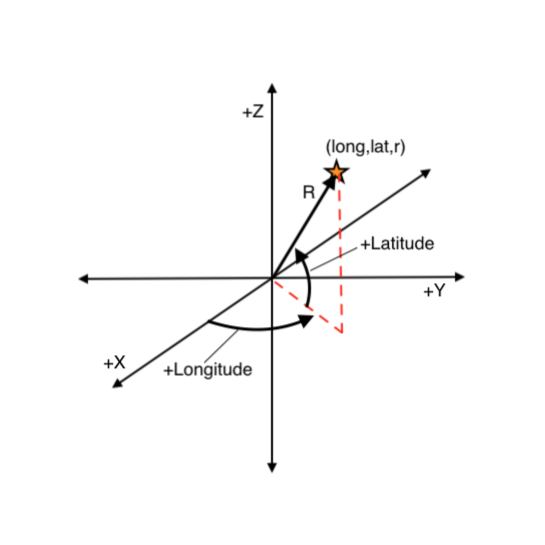
\includegraphics{diagrams/SphericalSpace.png}
  \end{minipage}

  \subsection{Standard 1D Coordinate Space}
  \label{sect:1DSpace}

  \vspace{-3cm}
  \begin{minipage}{0.5\textwidth}
    \small
    \textbf{id}: \_STANDARD\_1D\_CoordSpace \newline
    Coordinate space comprised of 1 axis.
    
    \noindent \textbf{Axis1} \newline
    \indent id:  Standard\_1D\_Axis \newline
    \indent domainMin:  -Infinity \newline
    \indent domainMax:  +Infinity \newline
    \indent cyclic:  False \newline
    
    \normalsize
  \end{minipage}
  \begin{minipage}{0.5\textwidth}
    
\includegraphics{diagrams/Standard1DSpace.png}
  \end{minipage}

